% ============================================================================
% OpenEarth v2 — system + methods preprint (arXiv style).
% Build: latexmk -pdf paper.tex   (see Makefile)
% All quantitative claims trace to committed repo artifacts; see the
% "Data and software availability" section for the mapping.
% ============================================================================
\documentclass[11pt]{article}

\usepackage[margin=1.1in]{geometry}
\usepackage[utf8]{inputenc}
\usepackage[T1]{fontenc}
\usepackage{newtxtext,newtxmath}
\usepackage{microtype}
\usepackage{amsmath}
\usepackage{graphicx}
\usepackage{booktabs}
\usepackage{multirow}
\usepackage[round,authoryear]{natbib}
\usepackage{xcolor}
\usepackage{tikz}
\usetikzlibrary{arrows.meta,positioning,fit}
\usepackage[font=small,labelfont=bf]{caption}
\usepackage[colorlinks=true,linkcolor={blue!50!black},citecolor={blue!50!black},urlcolor={blue!50!black}]{hyperref}

\graphicspath{{figures/}}

\newcommand{\dR}{\Delta R}
\newcommand{\dOm}{\Delta\Omega}
\newcommand{\perh}{\ensuremath{\,\mathrm{t\,h^{-1}}}}
\newcommand{\kgh}{\ensuremath{\,\mathrm{kg\,h^{-1}}}}
\newcommand{\molm}{\ensuremath{\,\mathrm{mol\,m^{-2}}}}
\newcommand{\code}[1]{\texttt{\small #1}}

\title{\textbf{OpenEarth: an open-source system for satellite-based
environmental analysis with a measurement-first Sentinel-2 methane
detection suite}}

\author{Benedict von Schubert\\[2pt]
\small Faculty of Physics and Astronomy, Heidelberg University\\
\small \texttt{benedictvonschubert@gmail.com}}

\date{\small July 2026 \;\textperiodcentered\; preprint describing OpenEarth~v2 (development phase~8)}

\begin{document}
\maketitle

\begin{abstract}
\noindent
Satellite detection of methane super-emitters has matured into
operational monitoring, but the tooling landscape remains split between
closed industrial pipelines and single-purpose research code. We present
\textbf{OpenEarth}, an open-source (MIT) full-stack system for
interactive satellite-based environmental analysis --- a unified
multi-mission data catalog, map platform, time-series/export/timelapse
machinery, and an embeddings explorer --- whose centerpiece is a
\emph{measurement-first} Sentinel-2 methane detection suite. The suite
independently reimplements the multi-band single-pass and multi-pass
(MBSP/MBMP) retrievals of \citet{varon2021} on its own line-by-line
lookup table, quantifies emissions by integrated mass enhancement with a
seeded joint Monte Carlo error budget, and attaches machine-checkable
diagnostic flags to every detection. Plume footprints are bit-for-bit
invariant to recalibration of the reporting lookup table. A 17-event
intercomparison with published Sentinel-2 quantifications (13 quantified)
is consistent with no aggregate offset --- median ratio 1.00, though the
$n{=}13$ bootstrap intervals are wide --- but shows a factor
${\approx}2.8$ log-scatter and no per-event rank skill, much of which is
anticipated by an empirical detection floor measured on 35 plume-free
scene pairs (pooled $24.6\perh$). A U-Net candidate ranker trained on CH4Net is evaluated
under a leakage-controlled protocol (scene-level $F_1$ 0.571 vs.\ 0.416
for the physics baseline), with its label-inheritance limits stated. Two
pre-registered design hypotheses were tested, refuted, and kept: adding
interfering-gas and solar-spectrum physics changed the forward model by
only ${\sim}1.6\,\%$, and a median-composite reference failed to rescue
the persistent-emitter case. Every headline number of the
single-reference pipeline is reproducible from committed artifacts; we
argue that this negative-result-preserving engineering discipline, more
than any individual algorithm, is the transferable contribution.
\end{abstract}

% ===========================================================================
\section{Introduction}\label{sec:intro}

Methane is responsible for roughly a quarter to a third of present-day
anthropogenic warming, and a disproportionate share of mitigable emissions is
concentrated in a small population of point-source ``super-emitters,''
predominantly in the oil and gas sector \citep{jacob2022,lauvaux2022}.
Because a vented well or an unlit flare can often be fixed within days of
being found \citep{irakulis2022}, satellite instruments that can
\emph{find and quantify} individual plumes have become a central
mitigation technology. A well-established tiering has emerged: global
mappers such as TROPOMI locate persistent hotspots at
${\sim}7\,\mathrm{km}$ resolution \citep{veefkind2012,lorente2021,
schuit2023}, while high-resolution imagers localize the responsible
facility --- among them, remarkably, the general-purpose Sentinel-2
mission \citep{drusch2012}, whose two shortwave-infrared bands turn out to
be usable as a crude two-channel methane spectrometer
\citep{varon2021,gorrono2023,ehret2022}.

The methods for Sentinel-2 point-source retrieval are published in detail,
and several operational systems exist --- Kayrros' multi-temporal pipeline
\citep{ehret2022}, the UNEP International Methane Emissions Observatory's
MARS system with its MARS-S2L deep-learning detector
\citep{allen2025mars}, and commercial platforms. What is harder to find is
an \emph{integrated, open, end-to-end system}: one tool that spans
interactive data browsing, physics retrieval, uncertainty quantification,
cross-instrument evidence, machine-learning triage, and honest reporting
of what a retrieval can and cannot support. Research code released with
methods papers is typically single-purpose; industrial pipelines are
closed; and the accuracy claims attached to satellite methane
quantification in general have been shown to deserve caution --- in the
only multi-system single-blind test to date, 95\,\% confidence intervals
contained the metered truth just 52--70\,\% of the time
\citep{sherwin2024}.

This paper describes \textbf{OpenEarth~v2}, an open-source system that
attempts to fill that gap, and documents the methodology of its methane
suite to a standard where every headline number is checkable from the
repository alone. OpenEarth is a \emph{tool}, not a hypothesis test, and
this is a systems-and-methods paper in the tradition of platform
descriptions such as Google Earth Engine \citep{gorelick2017}. Its
contributions are:

\begin{enumerate}\itemsep2pt
  \item \textbf{An integrated open platform} (Sect.~\ref{sec:system}): a
  Python core library, FastAPI backend, and React/MapLibre frontend
  covering a unified multi-mission catalog (Sentinel-1/-2/-5P, EMIT,
  arbitrary user-registered Earth Engine collections), tiled browsing,
  time series, exports, a two-map compare view, a timelapse studio, and an
  explorer for the AlphaEarth satellite embedding fields
  \citep{brown2025alphaearth}.
  \item \textbf{An independent reimplementation and audit of the
  Sentinel-2 methane retrieval} (Sect.~\ref{sec:methane}): MBSP/MBMP
  fractional signals, its own line-by-line lookup table with committed
  provenance, robust plume masking that is provably decoupled from
  calibration changes, and integrated-mass-enhancement (IME)
  quantification with a seeded joint Monte Carlo error budget in which
  literature constants and own modeling choices are explicitly separated.
  \item \textbf{Measured rather than asserted performance}
  (Sect.~\ref{sec:eval}): reproduction of two documented super-emitter
  events; a 17-event intercomparison against published per-scene
  quantifications --- nothing is ever fitted to them --- with frozen,
  committed baselines for every algorithm version; and an empirical
  per-site detection floor obtained by running the identical pipeline on
  plume-free scene pairs.
  \item \textbf{A protocol-corrected ML tier} (Sect.~\ref{sec:ml}): a
  U-Net candidate ranker trained on CH4Net \citep{vaughan2024} under a
  license wall, with site-cluster grouped cross-validation, inner-fold
  early stopping and threshold selection, a label-quality gate, and an
  honest statement of what beating an MBMP-derived baseline on
  MBMP-guided labels does and does not mean.
  \item \textbf{Recorded negative results}: the hypothesis that the
  retrieval's ${\sim}23\,\%$ forward-model offset is dominated by missing
  interfering-gas/solar physics was tested and refuted
  (Sect.~\ref{sec:lut}); the hypothesis that a median-composite reference
  rescues recurrent emitters was tested and refuted
  (Sect.~\ref{sec:composite}). Both ship with their pre-registered
  predictions and A/B numbers.
\end{enumerate}

We deliberately claim no new retrieval physics: the scientific content of
the methane suite is an implementation, a verification audit, and an
honesty layer over published methods.

% ===========================================================================
\section{Related work}\label{sec:related}

\paragraph{Sentinel-2 point-source retrieval.}
\citet{varon2018} introduced the integrated mass enhancement (IME) method
for converting column plumes to emission rates at fine scales;
\citet{varon2021} demonstrated CH$_4$ retrieval from Sentinel-2's B11/B12
SWIR bands via multi-band (MBSP) and multi-temporal (MBMP) fractional
signals, with LES-calibrated effective winds. \citet{gorrono2023} analyzed
the method's error budget and detection limits, and published the
simulated-plume benchmark dataset (S2CH4) we adopt for future work
\citep{s2ch4_dataset}. \citet{ehret2022} industrialized multi-temporal
detection with a regression background over ${\sim}30$-date stacks ---
the design we treat as the literature's answer to reference selection
(Sect.~\ref{sec:composite}).

\paragraph{Operational monitoring.}
UNEP's IMEO operates MARS, whose Sentinel-2/Landsat detector MARS-S2L is
trained on ${\sim}87{,}000$ image pairs \citep{allen2025mars,
mars_s2l_dataset}; SRON's TROPOMI pipeline finds thousands of plumes per
year with a CNN + SVC two-stage detector \citep{schuit2023}. Every
operational system keeps humans in the loop for outward-facing claims ---
a design decision OpenEarth adopts (Sect.~\ref{sec:ml}). Blind testing
against metered releases \citep{sherwin2024} motivates our skepticism
toward uncertainty bands, including our own.

\paragraph{Learned detectors.}
CH4Net \citep{vaughan2024} trains a U-Net on hand-annotated Sentinel-2
plumes over Turkmenistan; MethaNet \citep{jongaramrungruang2022}
regresses emission rates directly from plume imagery; and
\citet{rouetleduc2024} report single-image detection with a vision
transformer at claimed sensitivities well below band-ratio methods.
OpenEarth's ML tier follows the candidate-ranker philosophy rather than
the autonomous-detector one.

\paragraph{Other instruments and platforms.}
The EMIT imaging spectrometer \citep{green2020} resolves individual plumes
at 60\,m and attributes them to facilities \citep{thorpe2023}, building on
the matched-filter point-source retrieval line demonstrated with PRISMA
\citep{guanter2021} and the detection-limit analysis of
\citet{cusworth2019}; OpenEarth consumes its published plume products as
independent evidence (Sect.~\ref{sec:emit}). All bulk data access runs through Google Earth
Engine \citep{gorelick2017}; winds come from ERA5/ERA5-Land
\citep{hersbach2020,munozsabater2021}; annual 64-band embedding fields
from AlphaEarth Foundations \citep{brown2025alphaearth} power the
similarity/change/clustering explorer.

% ===========================================================================
\section{System architecture}\label{sec:system}

\begin{figure}[tb]
\centering
\begin{tikzpicture}[
  font=\small,
  box/.style={draw=black!55, rounded corners=2pt, align=center,
              inner sep=5pt, fill=black!3, text width=11.2cm},
  ext/.style={draw=black!40, dashed, rounded corners=2pt, align=center,
              inner sep=4pt, fill=white},
  lbl/.style={font=\footnotesize\itshape, text=black!60},
  arr/.style={-{Stealth[length=2mm]}, black!60}
]
\node[box, minimum width=11.6cm] (web)
  {\textbf{\code{apps/web}} --- React + TypeScript + MapLibre~GL\\[1pt]
   \footnotesize Explore \textperiodcentered\ Compare \textperiodcentered\
   Methane Lab \textperiodcentered\ Timelapse Studio \textperiodcentered\
   Embeddings Explorer \textperiodcentered\ Settings};
\node[box, minimum width=11.6cm, below=14pt of web] (api)
  {\textbf{\code{packages/api}} --- FastAPI\\[1pt]
   \footnotesize REST + server-sent-event jobs \textperiodcentered\
   SQLite (WAL, append-only migrations) \textperiodcentered\
   one versioned disk cache \textperiodcentered\ ONNX inference (CPU)};
\node[box, minimum width=11.6cm, below=14pt of api] (core)
  {\textbf{\code{packages/core}} --- Python science library\\[1pt]
   \footnotesize dataset catalog \textperiodcentered\ EE providers +
   throttled client \textperiodcentered\ \emph{NumPy methane physics}
   \textperiodcentered\ pixel grids \textperiodcentered\ timelapse
   \textperiodcentered\ embeddings};
\node[box, right=10pt of web.east, anchor=west, minimum height=1.05cm,
      text width=2.6cm] (ml)
  {\textbf{\code{packages/ml}}\\ \footnotesize offline training\\
   \footnotesize (PyTorch)};
\node[ext, below=12pt of core, xshift=-3.6cm] (gee) {Google Earth Engine\\
  \footnotesize S1/S2/S5P/EMIT mirrors, ERA5};
\node[ext, below=12pt of core, xshift=+3.6cm] (daac) {NASA LP DAAC\\
  \footnotesize EMIT V002 via \code{earthaccess}};
\draw[arr] (web.south) -- (api.north)
  node[midway, right=2pt, lbl] {generated typed client, SSE};
\draw[arr] (api.south) -- (core.north)
  node[midway, right=2pt, lbl] {thin routers, services off event loop};
\draw[arr] (gee.north) -- ([xshift=-3.6cm]core.south);
\draw[arr] (daac.north) -- ([xshift=+3.6cm]core.south);
\draw[arr, dashed] (ml.south) |- ([yshift=6pt]api.east)
  node[pos=0.75, above, lbl] {ONNX, out-of-band};
\end{tikzpicture}
\caption{OpenEarth v2 architecture. The core library contains no UI or web
dependencies and all science-critical mathematics runs on plain NumPy
arrays (offline-testable); Earth Engine is used for browsing, chip
fetching, and bulk reduction only. The ML training package is fully
offline and communicates with the serving stack only through an exported
ONNX artifact.}
\label{fig:arch}
\end{figure}

OpenEarth is a uv-workspace monorepo with three runtime components and one
offline component (Fig.~\ref{fig:arch}); \code{docker compose up} serves
the full stack. Five ground rules shape everything and are enforced
mechanically where possible:

\begin{enumerate}\itemsep2pt
\item \textbf{Earth Engine for browsing and bulk reduction; NumPy for
physics.} Everything science-critical operates on plain arrays
(``chips'') fetched via \code{computePixels} on explicit EPSG:4326 grids,
so the entire retrieval is unit-testable offline. The suite currently runs 590 offline tests with
zero network calls; live Earth-Engine tests are opt-in and never run in
CI.
\item \textbf{The core library has no UI or serving dependencies}, and the
training package's PyTorch never appears in the serving path --- both
enforced by dedicated tests.
\item \textbf{All blocking Earth-Engine round-trips pass through one
throttled, retrying client} (global semaphore + exponential backoff on
quota/transient errors), designed against EE's practical limits (tile-URL
lifetime, ${\sim}48\,$MB \code{computePixels} responses, concurrent
request quotas).
\item \textbf{One new dataset requires zero new code}: datasets are
declarative catalog entries (frozen \code{DatasetSpec}/\code{ProductSpec}
models), and any public Earth-Engine \code{ImageCollection} can be
registered at runtime from a TOML file. Derived products that need
two-window ``compare'' semantics (e.g.\ burn-scar dNBR, flood VV change)
declare \code{needs\_ref} and flow through a generic pre/post pipeline.
\item \textbf{Results are versioned and cache-keyed}: a single disk cache
keyed by canonical-JSON SHA-256 that includes a global
\code{ALGO\_VERSION} (currently 6), so no stale scientific result can
survive an algorithm change.
\end{enumerate}

The API layer adds an in-process job manager (SQLite WAL, append-only
schema migrations, cooperative cancellation) that streams progress over
server-sent events --- long-running analyses (time series, exports,
methane detections, ML scans, timelapse renders) are jobs with live
partial results. The web client is a thin imperative MapLibre binding with
a strict no-refetch rule for layer controls, a shared two-concept time
model (a compositing \emph{window} and a scanning \emph{period}), and
generated API types that CI checks against the server schema. Beyond the
methane lab, the platform ships interactive time series with progressive
coarse-to-fine fill, GeoTIFF/PNG/CSV export for every product, a
two-map compare view, a timelapse studio with resilient rendering
(a mid-render failure costs one frame, not the render; cancellation keeps
a playable partial), a GPU wind-particle layer fed by ERA5, and an
AlphaEarth embeddings explorer (cosine similarity to a clicked seed,
year-over-year change, seeded $k$-means clustering) with the dataset's
CC-BY attribution displayed wherever a layer is visible.

% ===========================================================================
\section{The methane detection suite}\label{sec:methane}

\begin{figure}[tb]
\centering
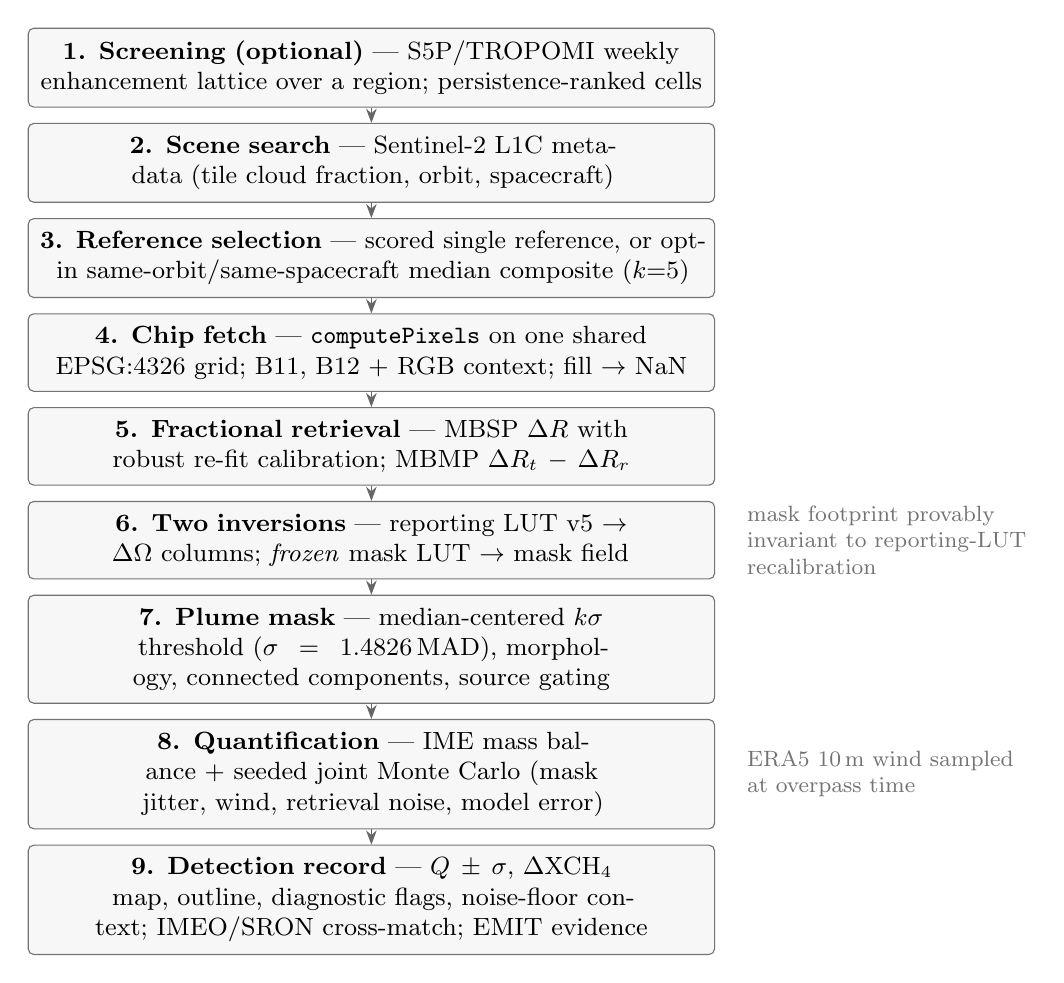
\begin{tikzpicture}[
  font=\small, node distance=5.5pt,
  stage/.style={draw=black!55, rounded corners=2pt, align=center,
               inner sep=4.5pt, fill=black!3, text width=8.4cm},
  side/.style={font=\footnotesize, text=black!55, align=left},
  arr/.style={-{Stealth[length=1.8mm]}, black!60}
]
\node[stage] (s1) {\textbf{1. Screening (optional)} --- S5P/TROPOMI weekly
  enhancement lattice over a region; persistence-ranked cells};
\node[stage, below=of s1] (s2) {\textbf{2. Scene search} --- Sentinel-2 L1C
  metadata (tile cloud fraction, orbit, spacecraft)};
\node[stage, below=of s2] (s3) {\textbf{3. Reference selection} --- scored
  single reference, or opt-in same-orbit/same-spacecraft median composite
  ($k{=}5$)};
\node[stage, below=of s3] (s4) {\textbf{4. Chip fetch} ---
  \code{computePixels} on one shared EPSG:4326 grid; B11, B12 + RGB
  context; fill $\to$ NaN};
\node[stage, below=of s4] (s5) {\textbf{5. Fractional retrieval} --- MBSP
  $\dR$ with robust re-fit calibration; MBMP $\dR_t - \dR_r$};
\node[stage, below=of s5] (s6) {\textbf{6. Two inversions} --- reporting
  LUT v5 $\to$ $\dOm$ columns; \emph{frozen} mask LUT $\to$ mask field};
\node[stage, below=of s6] (s7) {\textbf{7. Plume mask} --- median-centered
  $k\sigma$ threshold ($\sigma = 1.4826\,$MAD), morphology, connected
  components, source gating};
\node[stage, below=of s7] (s8) {\textbf{8. Quantification} --- IME mass
  balance + seeded joint Monte Carlo (mask jitter, wind, retrieval noise,
  model error)};
\node[stage, below=of s8] (s9) {\textbf{9. Detection record} --- $Q \pm
  \sigma$, $\Delta\mathrm{XCH_4}$ map, outline, diagnostic flags,
  noise-floor context; IMEO/SRON cross-match; EMIT evidence};
\foreach \a/\b in {s1/s2, s2/s3, s3/s4, s4/s5, s5/s6, s6/s7, s7/s8, s8/s9}
  \draw[arr] (\a.south) -- (\b.north);
\node[side, right=8pt of s8.east, anchor=west]
  {ERA5 10\,m wind sampled\\ at overpass time};
\node[side, right=8pt of s6.east, anchor=west]
  {mask footprint provably\\ invariant to reporting-LUT\\ recalibration};
\end{tikzpicture}
\caption{The cancellable detection pipeline implemented in
\code{methane/detect.py}. Steps 4--8 are pure NumPy and covered by the
offline test suite; every step contributes machine-readable diagnostic
flags to the final record.}
\label{fig:pipeline}
\end{figure}

The methane suite (Fig.~\ref{fig:pipeline}) follows \citet{varon2021}
end-to-end, with deviations that are individually declared and tested.
This section states the method compactly; the repository's methods
document carries the full derivations and per-decision rationale.

% ---------------------------------------------------------------------------
\subsection{Fractional-absorption retrieval (MBSP/MBMP)}\label{sec:retrieval}

Methane absorbs in Sentinel-2's B12 band (${\sim}2100$--$2280\,$nm) and
weakly in B11 (${\sim}1560$--$1660\,$nm). The multi-band single-pass
signal of a scene is
\begin{equation}
  \dR \;=\; \frac{c\,R_{12} - R_{11}}{R_{11}},
  \qquad
  c \;=\; \frac{\sum R_{11} R_{12}}{\sum R_{12}^2},
\end{equation}
with $R_{11}, R_{12}$ top-of-atmosphere reflectances (L1C, pinned
deliberately --- the retrieval literature calibrates against TOA) and $c$
the zero-intercept least-squares slope over valid pixels. A plume
depresses $R_{12}$ and drives $\dR$ negative. The slope is re-fit once
excluding pixels with $|\dR| > 1\sigma$ so that a real plume cannot bias
its own calibration; a unit test pins the failure mode this prevents. The
multi-band multi-pass signal subtracts a reference scene to cancel static
surface structure, $\dR_{\mathrm{MBMP}} = \dR_{\mathrm{target}} -
\dR_{\mathrm{reference}}$.

Both chips are fetched on the \emph{same} corner-origin EPSG:4326 grid, so
subtraction is element-wise by construction rather than after an explicit
warp. The grid contract is pinned by live-probe tests (pixel-center
sampling verified against \code{ee.Image.pixelLonLat} to $<10^{-5}$
degrees; nearest-neighbour band resampling verified empirically), and its
consequence is a registration \emph{hierarchy}: same-orbit references
resample onto essentially identical ground pixels, cross-orbit references
incur sub-pixel view-geometry shifts, and references from a different UTM
zone can shift by up to half a 20\,m pixel per band. The last case is
flagged (\code{cross\_tile\_reference}) rather than silently absorbed ---
one intercomparison event (permian) shows the resulting ${\sim}2\times$
over-estimate (Appendix~\ref{app:events}).

% ---------------------------------------------------------------------------
\subsection{Column conversion: a custom absorption LUT with committed
provenance}\label{sec:lut}

$\dR$ maps to a methane column enhancement $\dOm$ (mol\,m$^{-2}$) through
a precomputed lookup table (LUT) generated offline by a script whose
inputs are committed --- HITRAN line data \citep{gordon2022hitran} fetched through
HAPI \citep{kochanov2016hapi}, the ESA spectral response functions
\citep{esasrf2022}, TSIS-1 HSRS solar irradiance \citep{coddington2021},
and an AFGL water-vapor profile \citep{anderson1986afgl}. The forward
model is layered Beer--Lambert band transmittance without scattering: the
US Standard Atmosphere \citep{ussa1976} is split into 16 equal-mass layers
with per-layer absorber-weighted Voigt cross sections; the background
optical depth includes well-mixed CH$_4$ (0.65\molm)
and CO$_2$ (420\,ppm, a declared constant) and profile-integrated H$_2$O
(${\approx}14.2\,\mathrm{kg\,m^{-2}}$ precipitable water); the band weight
is $w(\nu) = \mathrm{SRF}_b(\nu)\, E_\nu(\nu)\,
e^{-\mathrm{AMF}\,\tau_{\mathrm{bg}}(\nu)}$, where $\mathrm{AMF} =
1/\cos\theta_{\mathrm{sun}} + 1/\cos\theta_{\mathrm{view}}$ is the
geometric air-mass factor and the solar spectrum is converted
per-wavenumber via the $\lambda^2$ Jacobian. The enhancement
$\dOm$ sits in the lowest 500\,m (the placement assumed by
\citealp{varon2021}), slanted by the same AMF.
Band signals combine as $m_{\mathrm{MBSP}} = (1 + m_{B12})/(1 + m_{B11}) -
1$, tabulated separately for Sentinel-2A and -2B (their B12 response
functions differ measurably; Fig.~\ref{fig:lut}a) over $\dOm \in [-0.5,
6.0]\molm$ and $\mathrm{AMF} \in [2, 4]$. Inversion is a monotonic
interpolation per pass; MBMP inverts each pass with its own AMF and
spacecraft before differencing, which handles mixed S2A/S2B pairs
correctly. Column enhancements convert to mixing-ratio units as
$\Delta\mathrm{XCH_4} = \dOm/\Omega_{\mathrm{air}} \times 10^9$ ppb with
$\Omega_{\mathrm{air}} = 3.567 \times 10^{5}\molm$.

\begin{figure}[tb]
\centering
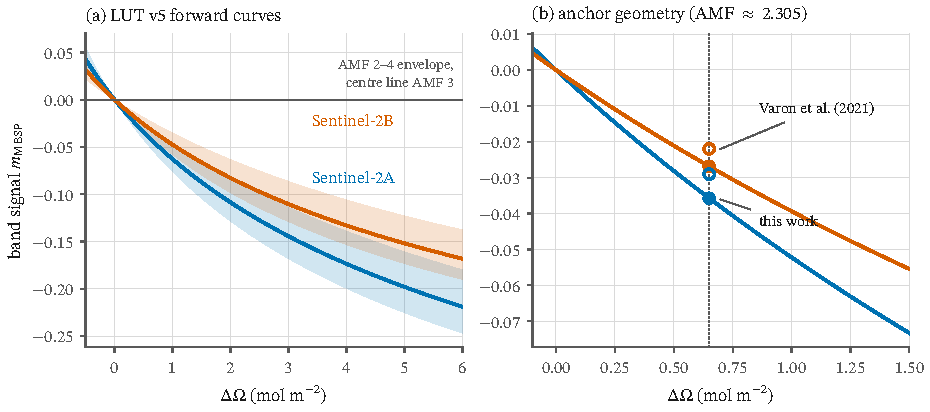
\includegraphics[width=\textwidth]{fig_lut.pdf}
\caption{The v5 absorption lookup table, plotted from the committed
artifact. (a) Forward band signal $m_{\mathrm{MBSP}}(\dOm)$ per
spacecraft; the shaded envelope spans air-mass factors 2--4. (b) At the
\citet{varon2021} anchor geometry ($40^\circ$ solar zenith, nadir view)
and a doubled background column ($\dOm = 0.65\molm$), our forward model
gives $-0.0357$ (S2A) and $-0.0268$ (S2B) against the published $-0.029$
and $-0.022$ --- a persistent ${\sim}23\,\%$ offset with the correct
inter-spacecraft ordering (Sect.~\ref{sec:lut}).}
\label{fig:lut}
\end{figure}

\paragraph{A refuted hypothesis, kept.}
The LUT's history is itself a result. An interim version (v2, single
effective layer) agreed with the Varon anchor to ${\sim}8\,\%$ --- by
\emph{error cancellation}, as replacing it with a resolved 16-layer
background (v3) revealed. The project roadmap then attributed the
remaining ${\sim}23\,\%$ anchor offset (Fig.~\ref{fig:lut}b) to the two
obvious spectroscopic omissions: interfering H$_2$O/CO$_2$ absorption and
solar-spectrum band weighting. Version 4 added both --- and moved the
anchor by only ${\sim}1.6\,\%$, refuting that attribution. The offset's
cause remains open (candidates: multiple scattering and aerosols, absent
from a Beer--Lambert model; sea-level surface pressure baked into the
background; deeper reference-model differences), and the v4 physics ships
for completeness and checkability, \emph{not} as an improvement on the
intercomparison aggregates
--- on the 17-event harness it is empirically indistinguishable from v3
(Sect.~\ref{sec:calibration}). Version 5 extends the $\dOm$ grid from 3.0
to 6.0\molm{} (bit-identical on the shared subgrid) so that surface-driven
MBSP blow-ups invert to large \emph{finite} columns instead of clamping at
the grid edge, and replaces the grid-edge exclusion with an explicit
inversion-validity bound (mask fraction with $|\dOm| \ge 3\molm$).

% ---------------------------------------------------------------------------
\subsection{Plume masking, decoupled from calibration}\label{sec:masking}

The plume footprint is thresholded on the $\dOm$ field of a \emph{frozen}
canonical inversion --- a pinned snapshot LUT used only for masking ---
rather than on the reporting LUT. The footprint is therefore invariant,
bit-for-bit, under reporting-LUT recalibration (enforced by a dedicated
test): v3$\to$v4$\to$v5 changed retrieved columns and rates but never
which pixels are called plume. The obvious LUT-independent alternative,
masking on raw $-\dR$, was implemented first and \emph{rejected after
diagnosis}: for MBMP it reintroduces surface-structure sensitivity (the
raw $\dR$ difference does not cancel co-saturated structure the way the
per-pass $\dOm$ difference does) and displaces the mask off the seeded
source entirely. The per-pass inversion is what localizes the plume ---
including, notably, through the S2A/S2B response difference for
mixed-spacecraft pairs --- so the design keeps it, with a fixed inversion.

Thresholding is $k\sigma$ on the positive enhancement tail, with $\sigma =
1.4826 \cdot \mathrm{MAD}$ about the median (robust, NaN-aware), optional
1-px binary opening, 8-connected components with a minimum area, and
selection of the component(s) intersecting a window around the queried
source (or containing the peak). ``No plume above threshold'' is a valid
empty result, not an error. Because masking and reporting use different
inversions, two distinct noise scales exist and are reported separately
($\sigma_{\mathrm{mask}}$ on the frozen field, $\sigma_{\mathrm{noise}}$
on the reporting field).

% ---------------------------------------------------------------------------
\subsection{Quantification: IME with a seeded joint Monte Carlo}\label{sec:ime}

Emission rate follows the IME mass balance
\citep{varon2018,varon2021}:
\begin{equation}
  Q \;=\; \frac{U_{\mathrm{eff}}}{L}\,\mathrm{IME},
  \qquad
  \mathrm{IME} = \sum_{\mathrm{mask}} \dOm \, A_{\mathrm{pix}}
  M_{\mathrm{CH_4}},
  \qquad
  L = \sqrt{n_{\mathrm{px}} A_{\mathrm{pix}}},
\end{equation}
with the LES-calibrated effective wind $U_{\mathrm{eff}} = 0.33\,U_{10} +
0.45\,\mathrm{m\,s^{-1}}$ and $U_{10}$ the ERA5 10\,m wind sampled at
overpass time (time-interpolated between bracketing hours, ERA5-Land with
an ERA5 water fallback). Uncertainty is a seeded joint Monte Carlo
($n{=}500$) perturbing four terms per draw: mask-threshold jitter ($k$
uniform over $\{1.5, \dots, 2.5\}$, with the five labelings precomputed),
wind (truncated normal), retrieval noise (a bootstrap of the off-plume
$\dOm$ population, recomputed excluding the mask so a plume cannot inflate
its own error bar), and a multiplicative mass-balance model error. The
reported $Q$ is the MC median, the band its standard deviation; identical
seeds give bit-identical results. Two properties of the band must be
understood when reading results. It is a \emph{precision} band --- the
spread of the four sampled terms --- and deliberately excludes known
systematics of comparable size: the ${\sim}23\,\%$ forward-model anchor
offset (Sect.~\ref{sec:lut}), AMF and geometry error, and
surface-albedo--retrieval covariance. This is exactly the
interval-overconfidence trap \citet{sherwin2024} document across nine
professional systems, and the band should be read accordingly. Second,
the scalar $\pm\sigma$ understates the asymmetry of the skewed $Q$
distributions involved; the full MC percentiles and histogram are stored
with every detection and shown in the applications.
Table~\ref{tab:budget} separates
literature constants from our own declared modeling choices --- the
position taken is that honest, documented constants beat irreproducible
pseudo-rigor.

\begin{table}[tb]
\centering\small
\caption{Error-budget constants: literature values vs.\ declared modeling
choices (all in \code{methane/constants.py}, cited inline).}
\label{tab:budget}
\begin{tabular}{@{}llp{7.1cm}@{}}
\toprule
Constant & Value & Provenance \\
\midrule
$U_{\mathrm{eff}} = \alpha U_{10} + \beta$ & $\alpha{=}0.33$,
$\beta{=}0.45\,\mathrm{m\,s^{-1}}$ & LES calibration of
\citet{varon2021} (literature; see the transfer caveat,
Sect.~\ref{sec:limitations}) \\
$\sigma_{U_{10}}$ floor & $1.5\,\mathrm{m\,s^{-1}}$ & \textbf{our choice}
--- a reanalysis wind error floor; Varon's GEOS-FP-vs-mesonet residuals
are not reproducible here \\
IME model error & $\mathcal{N}(1, 0.15)$ multiplicative & \textbf{our
choice} --- mass-balance model spread; the original LES hold-out is not
reproducible here \\
\bottomrule
\end{tabular}
\end{table}

% ---------------------------------------------------------------------------
\subsection{Reference selection and the composite-reference
experiment}\label{sec:composite}

MBMP needs a plume-free reference, and the published baseline never solved
selection --- \citet{varon2021} picked references by hand.
OpenEarth's default picker is metadata-scored (cloud fraction, time
distance, same-orbit and same-spacecraft preferences), excludes the
same-overpass adjacent tile (which images the same plume), and flags
suspected contamination by re-running plume detection on the reference
itself.

Phase 8 added an \textbf{opt-in composite reference}: up to $k{=}5$
same-orbit, \emph{same-spacecraft} reference chips combined by per-pixel
median upstream of an unchanged retrieval, with the reference pass
inverted at the median member AMF (a declared approximation, flagged when
the member spread exceeds one LUT grid step). The median's 50\,\%
breakdown point is the design idea: an intermittent plume must contaminate
the same pixels in half the members to survive. This is our own design,
literature-adjacent but distinct from \citet{ehret2022}'s regression
background, and it was evaluated with hypotheses fixed \emph{before} the
run against the frozen single-reference baseline
(Table~\ref{tab:composite}).

\begin{table}[tb]
\centering\small
\caption{Composite-reference A/B on the 17-event harness (LUT v5, seed 0).
Hypotheses were pre-registered; the headline hypothesis was refuted, so
the mode ships opt-in and default-off. Unlike the single-reference
baselines, the composite column records a single documented live run with
no frozen per-event artifact; its slope movement is dominated by one
event (korpezhe, Sect.~\ref{sec:composite}).}
\label{tab:composite}
\begin{tabular}{@{}lccc@{}}
\toprule
Aggregate & Single (v5 baseline) & Composite & $\Delta$ \\
\midrule
Through-origin slope & 1.105 & 1.962 & $+0.857$ \\
Median ratio         & 0.996 & 0.955 & $-0.041$ \\
Robust log-scatter   & 0.441 & 0.425 & $-0.016$ \\
Theil--Sen slope     & 0.124 & 0.168 & $+0.044$ \\
Spearman $\rho$      & 0.088 & 0.070 & $-0.018$ \\
$n$ quantified       & 13    & 12    & --- \\
\bottomrule
\end{tabular}
\end{table}

The decisive finding is negative: for the textbook persistent-emitter
failure case (libya-sirte, published $14.7\perh$, single-reference
retrieval $1.7\perh$ because the reference itself was emitting), the
composite moved the estimate from 1.72 to only $1.76\perh$. A
\emph{recurrent} emitter contaminates more than half of its nearby
same-orbit candidates, so the median's breakdown point buys nothing ---
the composite addresses intermittent contamination, not persistence.
One event (korpezhe) became strictly worse --- 10.95 to $162\perh$ ---
because its documented hand-picked plume-free reference was replaced by
auto-selected members sharing the site's contamination; that single point
dominates the slope movement in Table~\ref{tab:composite}, whose columns
also differ by one event (one fewer quantifies under the composite). The
pre-registered secondary hypothesis --- scatter drops at homogeneous
sites --- was assessed only on the full-set log-scatter, which moved
marginally ($-0.016$); no homogeneous-subset statistic was computed.
Consequently the composite ships default-off, no baseline was re-frozen
around it, and the literature's regression-background design remains the
recorded upgrade path.

% ---------------------------------------------------------------------------
\subsection{Screening and validation tiers}\label{sec:tiers}

A TROPOMI screening tier ranks region cells by persistent weekly XCH$_4$
enhancement over a per-pixel median background (one reduction per week;
$z$-scored against all cell-weeks) before any Sentinel-2 retrieval is
spent. Beyond the product's valid-range masking, no albedo- or
aerosol-artifact screening is applied, although persistent artifacts are
known to mimic enhancements \citep{lorente2021,schuit2023} --- the tier
is triage only, and this susceptibility is declared. A validation
importer ingests public event inventories (IMEO, SRON) from CSV/GeoJSON
with explicit rate units --- no unit guessing, out-of-range rows dropped
and counted --- and cross-matches detections by haversine distance and
time (\emph{confirmed} within 15\,km and $\pm$14\,d; \emph{plausible}
within $\pm$60\,d). The radii are deliberately loose co-location for
review triage; in a dense basin 15\,km spans many facilities, so a match
is corroboration, not facility-level attribution. \emph{Contradicted} is
never assigned automatically: event lists prove presence, not absence.

% ---------------------------------------------------------------------------
\subsection{EMIT: independent evidence, not a second
detector}\label{sec:emit}

The EMIT imaging spectrometer \citep{green2020,thorpe2023} resolves plumes
at 60\,m. OpenEarth attaches EMIT's published plume-complex products to
detections as \emph{independent evidence from another instrument} ---
never as detection rows of its own, and decoupled from the physics/ML
feed. Two sources with different coverage are handled behind one model: a
frozen Earth-Engine mirror of the V001 product (2022-08-10 to 2024-10-26,
upstream-decommissioned) and the live LP DAAC V002 GeoJSON metadata (which
adds an emission-rate estimate), each plume provenance-tagged; windows
straddling the boundary query both and de-duplicate. Cross-match is
$\le$5\,km and $\le$3\,d. Because V001 and V002 rasters are not
numerically identical, quantitative comparisons never mix versions.

Units convert for order-of-magnitude context only: EMIT reports
ppm$\cdot$m, which relates to column density through the surface air
number density, $1\,\mathrm{ppm{\cdot}m} \approx 4.3\times10^{-5}\molm$ at
US-Standard surface conditions ($\pm{\sim}15\,\%$ over plausible surface
$P/T$). On a matched 2023 Permian super-emitter (EMIT overpass 2023-06-16;
our nearest Sentinel-2 MBMP retrieval $+3$\,d), both instruments
independently flag an extreme column-scale event at the same location
while the masked-mean columns differ by ${\sim}1.5$ orders of magnitude
--- expected across a 3-day gap, different masks, and our known
forward-model gap, and precisely why this tier is corroboration, never a
calibration reference.

% ===========================================================================
\section{Evaluation of the physics tier}\label{sec:eval}

\subsection{Reproduction of documented events}\label{sec:gate}

The suite's original exit gate reproduces two documented super-emitter
events against live Earth Engine (Table~\ref{tab:gate}). Values agree
within $\pm50\,\%$ with published quantifications; the wide Korpezhe band
is genuine plume-footprint ambiguity for an intermittent source with a
different-date reference, reported rather than tuned away.

\begin{table}[tb]
\centering\small
\caption{Two-event reproduction gate (LUT v3 era; MC bands are 1$\sigma$).
Published values from \citet{varon2021}. These v3-era numbers are
retained as the original exit gate; Korpezhe's current v5 retrieval
appears in Table~\ref{tab:events}.}
\label{tab:gate}
\begin{tabular}{@{}llll@{}}
\toprule
Event & Method & Published & This work \\
\midrule
Korpezhe (TM), 2018-06-19 & MBMP & $11.2 \pm 5.2\perh$ & $13.7 \pm
22.7\perh$ \\
Hassi Messaoud (DZ) blowout, 2019--2020 & MBSP, 3-scene mean &
$9.3 \pm 5.5\perh$ & $8.5\perh$ (6.8, 13.2, 5.4) \\
\bottomrule
\end{tabular}
\end{table}

\subsection{Consistency with published quantifications}\label{sec:calibration}

\begin{figure}[tb]
\centering
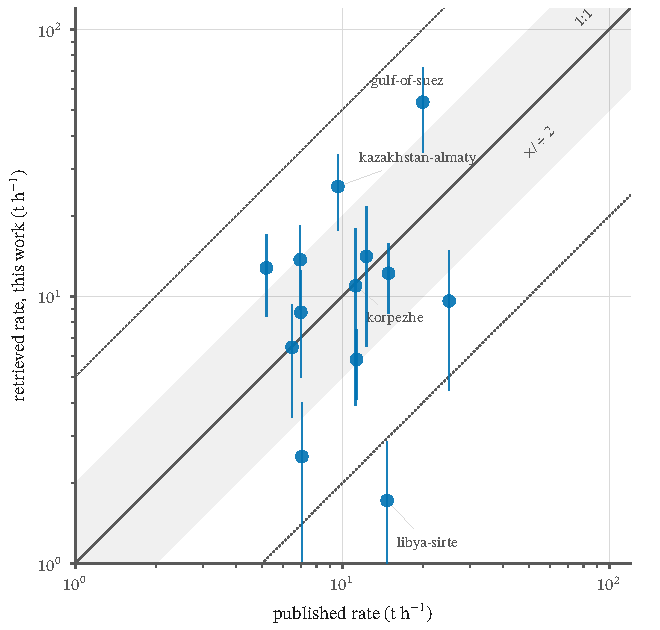
\includegraphics[width=0.62\textwidth]{fig_calibration.pdf}
\caption{Retrieved vs.\ published emission rates for the 13 quantified
events of the frozen v5 baseline (log--log; bars are MC
1$\sigma$; shading spans a factor of 2, dashed lines a factor of 5).
The aggregate shows no net offset (median ratio 1.00; the $n{=}13$
bootstrap intervals are wide, Sect.~\ref{sec:calibration}) with a factor
${\approx}2.8$ robust log-scatter. The reference-contamination diagnostic
fires on 12 of 13 events --- and on all 27 plume-free noise-floor pairs
that produced a detection (Sect.~\ref{sec:floor}) --- a deliberately
conservative prompt for review, not a discriminator. The
libya-sirte outlier is the persistent-emitter reference-contamination
failure discussed in Sect.~\ref{sec:composite}.}
\label{fig:calibration}
\end{figure}

A harness runs the full \code{analyze} pipeline over 17 same-scene
Sentinel-2 events --- IMEO MARS-S2L per-scene quantifications
\citep{mars_s2l_dataset} plus the Korpezhe anchor of \citet{varon2021},
spanning ${\sim}5$--$25\perh$ --- and regresses retrieved against
published rates (Fig.~\ref{fig:calibration}; Appendix~\ref{app:events}).
Two scope statements come first. This is an \emph{intercomparison}, not a
calibration: nothing is ever fitted to the published rates (a standing
project rule), and 12 of the 13 quantified reference values are
themselves Sentinel-2 IME retrievals from the same method family --- so
agreement measures consistency with community retrievals, not accuracy
against true flux, which only the planned LES-truth benchmark can measure
(Sect.~\ref{sec:future}). Second, the aggregates are conditional on
quantification: 13 of 17 events quantify, with three documented validity
exclusions and one non-detection (Appendix~\ref{app:events}) --- a 4/17
non-quantification rate on documented super-emitters that is itself a
performance number. Every event's published value derives from the same
acquisition we analyze; TROPOMI-scale weekly lists are excluded by design
(7\,km pixels measure source variability, not per-scene consistency).
Aggregates for the three LUT generations are frozen as committed baselines
(Table~\ref{tab:aggregates}).

\begin{table}[tb]
\centering\small
\caption{Intercomparison aggregates across LUT versions (seed 0, $n{=}500$
MC). Masks are identical across versions by construction
(Sect.~\ref{sec:masking}); v5 quantifies fewer events because its
inversion-validity bound excludes two additional surface-dominated
retrievals (ahvaz, gulf-of-thailand). Every row is a committed JSON
baseline.}
\label{tab:aggregates}
\begin{tabular}{@{}lccccc@{}}
\toprule
& $n$ & Through-origin slope & Theil--Sen slope & Median ratio &
Robust log-scatter \\
\midrule
LUT v3 & 15 & 1.027 & 0.200 & 0.967 & 0.424 \\
LUT v4 & 15 & 1.042 & 0.190 & 0.972 & 0.413 \\
LUT v5 & 13 & 1.105 & 0.124 & 0.996 & 0.441 \\
\bottomrule
\end{tabular}
\end{table}

Three findings deserve emphasis, all of them things a less
measurement-driven port would have missed:

\paragraph{MBSP fails structurally over heterogeneous surfaces.}
Single-scene MBSP has no reference to cancel static surface structure;
over heterogeneous terrain, coherent bright/dark regions invert to huge
columns and connected components engulf them into multi-thousand-pixel
false plumes of hundreds of $\mathrm{t\,h^{-1}}$ (one event: $473\perh$
from a 9{,}561-pixel mask, 76\,\% beyond the inversion-validity bound).
This is why \citet{varon2021} prefer MBMP; the harness therefore defaults
every event to MBMP with a pinned plume-free reference --- the reference
pass carries the same surface structure, and co-located saturation cancels
in the $\dOm$ difference (the same event under MBMP: $14.1 \pm 7.6\perh$
vs.\ $12.3\perh$ published). Retrievals whose mask exceeds 20\,\%
out-of-validity fraction
are excluded (documented, and blind to the published value), never
silently.

\paragraph{The aggregate is consistent; individual events are not.}
The v5 central tendency shows no net offset --- median ratio 0.996 ---
but with $n = 13$ the statistics are weak: a bootstrap over events
(reproducible from the committed baseline) gives 95\,\% intervals of
0.51--1.98 on the median ratio, 0.54--1.91 on the through-origin slope,
and 0.09--0.64 on the robust log-scatter of 0.44 (a factor
${\approx}2.8$). The scatter has known, named causes (reference quality
at recurrent emitters; the published rates embed different wind data than
our ERA5; single-scene surface heterogeneity) and is reported instead of
chased per-event.
The slope--median split (1.105 vs.\ 0.996) is recorded as an open
observation, not a demonstrated rate dependence: the gap sits well inside
both bootstrap intervals, it is driven by a few large \emph{retrievals}
(gulf-of-suez, kazakhstan-almaty) rather than by the largest published
emitters (the largest, turkmenistan-south, is \emph{under}-estimated),
and the null rank correlation cautions against reading any trend.
Candidate mechanisms (mask-size growth at high IME, wind-error scaling,
the IME's heavy upper tail) are documented, unresolved.

\paragraph{The event set sits at the pipeline's own noise floor.}
The quantified events' published rates (5.2--25.1\perh) lie at or near
--- mostly below --- the pooled $24.6\perh$ detection floor of
Sect.~\ref{sec:floor}; at Hassi Messaoud, a $7.0\perh$ event is compared
against a $6.6\perh$ site floor. A substantial part of the observed
scatter --- and of the null rank skill below --- is therefore
\emph{predicted} by the floor rather than diagnostic of the retrieval
alone, and over this narrow dynamic range a rank test has little power
even for a well-calibrated system: injecting the observed 0.44\,dex
scatter onto the 13 published rates (a seeded simulation, reproducible
from the committed baseline) yields median $\rho \approx 0.4$ and rejects
at $\alpha = 0.05$ only 29\,\% of the time. The two sections measure the
same limitation from two sides.

\paragraph{Per-event rank skill is indistinguishable from zero.}
Spearman $\rho = 0.09$ ($p = 0.78$, $n = 13$) between published and
retrieved rates --- partly a property of this event set (above), partly
of the retrieval. The honest three-part statement, propagated into the
UI: the aggregate is consistent with community retrievals, within wide
$n{=}13$ intervals; a single retrieved rate is an order-of-magnitude
estimate; and ranking two sources by retrieved $Q$ is unsupported. We consider stating this plainly more valuable than
the slope itself, and note that even purpose-built systems show sobering
blind-test interval coverage \citep{sherwin2024}.

Finally, the v5 grid extension produced a genuine per-event correction:
the Korpezhe retrieval, edge-clamped under v4, un-clamps from 5.7 to
$11.0\perh$ --- onto its $11.2\perh$ published anchor --- while the
\emph{aggregate} numbers moved by less than the scatter in split
directions (median toward 1, slopes away). v5 was adopted for correct
finite-column physics and the tightened validity exclusion, explicitly
\emph{not} as a demonstrated aggregate gain: the estimator split is
structurally forced when a residual distribution straddles unity, and
pretending otherwise would be over-claiming.

\subsection{An empirical detection floor}\label{sec:floor}

\begin{figure}[tb]
\centering
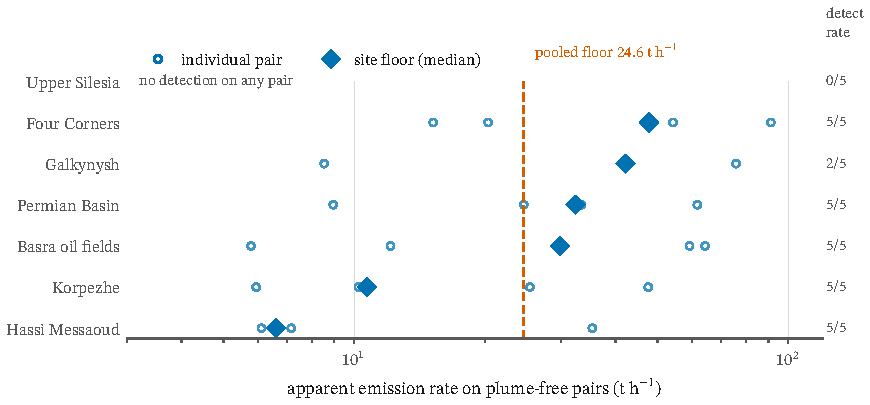
\includegraphics[width=0.9\textwidth]{fig_noise_floor.pdf}
\caption{Empirical noise floor, from the committed v1 artifact: the
identical \code{analyze} pipeline run on five presumed-plume-free scene
pairs per seeded site. Open circles are individual pairs' apparent rates;
diamonds the per-site median floor; 27 of 35 pairs (77\,\%) yield a
quantifiable ``detection.'' At recurrent-emitter sites the floor absorbs
real residual emission, making it an upper bound on trustworthiness ---
the conservative direction.}
\label{fig:floor}
\end{figure}

Detection-limit claims for Sentinel-2 methane retrievals span
$0.2$--$10\perh$ in the literature depending on method and surface
\citep{varon2021,gorrono2023,rouetleduc2024}; purpose-built imaging
spectrometers reach substantially lower \citep{cusworth2019}. Rather than
assert a number,
OpenEarth \emph{measures} its own floor: the identical detection pipeline
(same thresholds, same MC) is run on seeded-random, presumed-plume-free
scene pairs at each built-in site, and the per-site floor is the median
apparent rate of these pure-noise ``detections''
(Fig.~\ref{fig:floor}). The results are sobering and site-dependent:
$6.6\perh$ at the best arid site (Hassi Messaoud), $30$--$48\perh$ over
heterogeneous terrain, a pooled floor of $24.6\perh$, and 77\,\% of
plume-free pairs yielding a quantifiable component at default settings. A
``detection'' near the floor is as likely retrieval noise as signal, and
the applications serve this context with every detection
(\code{below\_noise\_floor}). Two caveats bound the floor itself. It is a
median of the \emph{detected} pairs only: at a 5/5 detect rate it marks
roughly the 50\,\%-false-alarm point, but at lower detect rates it is an
upper percentile of the pair distribution (Galkynysh's floor is a median
of two values), and a percentile-based floor is a natural refinement.
And medians of at most five pairs carry sampling uncertainty of tens of
percent. Two consequences follow: first, the
${\sim}23\,\%$ LUT anchor offset is second-order next to a floor of tens
of $\mathrm{t\,h^{-1}}$ at most sites; second, most literature
detection-limit numbers are not directly comparable to an
operationally-thresholded pipeline's real-world floor --- which is
precisely why we publish the measurement methodology alongside the number.

% ===========================================================================
\section{The ML tier: a candidate ranker under a license
wall}\label{sec:ml}

The ML tier is a U-Net that \emph{ranks candidate scenes for human
review}; it feeds the same detection feed as the physics tier, never
auto-confirms, and changes no reported column or rate. This mirrors
operational practice everywhere --- Kayrros validates detections manually,
IMEO keeps analysts in the loop, SRON separates detection from
verification \citep{ehret2022,allen2025mars,schuit2023}.

\subsection{Training data, license wall, and metadata recovery}

Training uses CH4Net \citep{ch4net_dataset,vaughan2024}: 925 hand-annotated
plume masks over 23 Turkmenistan oil-and-gas sites. The dataset
is CC-BY-NC-ND and gated; consequently \emph{nothing derived from it is
ever committed or published} --- no chips, masks, weights, ONNX file, or
manifest. All derivatives live outside version control, the trained model
ships out-of-band, and the ND term is recorded in the model manifest as a
block on any public deployment of the weights. The evaluation numbers
below are aggregate metrics, which is all the repository retains.

Two engineering problems shaped this tier. First, \emph{train/serve
consistency}: CH4Net tiles are Sentinel-Hub L1C interpolated to 10\,m,
while our scan pipeline sees Earth-Engine L1C at 20\,m --- so chips are
rebuilt through our own fetch path at 20\,m and the published masks
regridded, guaranteeing the network sees the same distribution in training
and serving. Second, the public release strips all scene metadata (tiles
are named by opaque integers), so a self-service recovery pipeline
reconstructs each tile's footprint and date: offline content-correlation
clustering, normalized-cross-correlation geolocation against site-anchored
composites (median centre error ${\sim}10$\,m against published
coordinates), and per-overpass date matching with a hard train/test
split-year prior. Site assignments are independently validated by rank
agreement with the paper's per-site plume statistics. Under an asymmetric
usability policy --- a positive needs a confident date (a mis-dated
positive is label noise), a negative only needs a plume-free scene ---
10{,}395 of 10{,}983 tiles are usable, at the cost of confident dates for
only 409 of 997 positives, recorded as the main cost of working from the
metadata-stripped release. The asymmetry leaves a residual noise channel
of its own: a mis-dated negative at a recurrent-emitter site can contain
an unannotated plume, accepted as label noise on the majority class.

\subsection{Physics-informed channels and a leakage-controlled
protocol}\label{sec:mlprotocol}

The network's five input channels are built by the \emph{same} core-library
function at training and scan time (byte-identical, enforced):
the MBMP and MBSP $\dR$ fields, the B12/B11 ratio, and the two raw SWIR
reflectances. The $\dR$ channels sit upstream of the LUT, so trained
models remain valid across LUT recalibrations. Channels are
robust-standardized with statistics frozen into the model manifest; chips
are reflect-padded identically in training and serving.

The evaluation protocol was rebuilt once --- and the original numbers
retired --- after an internal review found three defects: folding by raw
site (neighbouring pads leak ground truth across folds), early stopping on
the evaluation fold, and a single untuned operating point. The corrected
protocol (v2) merges sites within 5\,km into clusters before 5-fold
grouped cross-validation (23 sites $\to$ 11 clusters, with a hard guard
aborting on any cross-fold footprint overlap), holds out an inner
validation cluster within each training fold for both early stopping and
probability-threshold selection (the evaluation fold is touched exactly
once, by a frozen model at a pre-selected threshold), gates out positives
whose own MBMP signal integrates to a net-negative column (69 of the 395
evaluation-set positives, 17.5\,\% --- labels contradicting the physics
they were drawn from; 395 of the 409 recovered-confident positives enter
evaluation), and
sweeps operating points on \emph{both} sides, reporting the baseline's
evaluation-oracle best-$k$ as an upper bound that favours it.

\begin{figure}[tb]
\centering
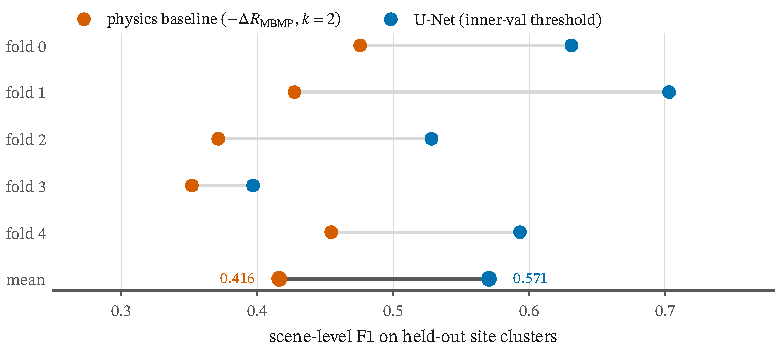
\includegraphics[width=0.8\textwidth]{fig_ml_eval.pdf}
\caption{Scene-level $F_1$ on held-out site clusters, per fold and mean,
from the committed v2 evaluation artifact: U-Net at the inner-validation
threshold vs.\ the $-\dR_{\mathrm{MBMP}}$ physics baseline at the pipeline
default $k{=}2$. The baseline's evaluation-oracle best-$k$ mean is 0.437.
The model beats its per-fold baseline in all five folds and clears the
aggregate gate ($0.571 \ge 0.416$).}
\label{fig:ml}
\end{figure}

The model beats the physics baseline, 0.571 vs.\ 0.416 mean scene-level
$F_1$ (Fig.~\ref{fig:ml}) --- \emph{lower} than the retired protocol-invalid
figure (0.597), which is the point: the earlier number was
inflated by exactly the defects the protocol now controls. Four caveats
bound the meaning. (i) CH4Net's masks were annotated with MBMP guidance,
so beating an MBMP-derived baseline on MBMP-guided labels demonstrates
better \emph{annotation agreement} --- a better candidate ranker --- not
an ability to see plumes MBMP cannot. (ii) 91.4\,\% of kept positive
labels have nominal rates below the Sect.~\ref{sec:floor} pooled noise
floor; the model largely reproduces annotations at rates the physics tier
calls indistinguishable from noise. (iii) 256 of 617 target scenes still
contribute chips to more than one fold (same acquisition, different pads)
--- a declared residual leakage channel. (iv) All sites are Turkmenistan
oil-and-gas; cluster-held-out CV controls intra-region leakage, not
geography, and the UI says so wherever scan results appear.

At serving time the exported ONNX model (dynamic input size,
${\sim}16$\,ms per chip on CPU) walks a site's scenes, and any scene with
candidates becomes a detection row marked as a point-estimate-only
candidate: a single-pass rate with no MC band, noise-floor context
attached, and a tri-state physics-agreement field (\emph{agree} /
\emph{physics-found-nothing} / \emph{physics-not-run}) computed at read
time --- deliberately not collapsing ``physics hasn't run'' into
``disagreement.'' The ML scan intentionally keeps the single-reference
picker even when the composite mode exists, because the training
distribution used single references and channel parity outranks
feature parity.

% ===========================================================================
\section{Limitations}\label{sec:limitations}

Most limitations have been quantified above; we collect the structural
ones.

\begin{itemize}\itemsep2pt
\item \textbf{Attribution, not identification.} Two SWIR bands cannot
spectrally fingerprint methane; a $\dR$ anomaly is \emph{attributed} to
CH$_4$, not proven to be it. Sentinel-2 has no usable band for any other
trace gas, which is also why independent EMIT evidence
(Sect.~\ref{sec:emit}) matters.
\item \textbf{No scattering physics.} The forward model is Beer--Lambert;
multiple scattering and aerosols are absent, sea-level surface pressure is
baked in (high-elevation sites are biased), and the ${\sim}23\,\%$ anchor
offset remains unattributed after two refuted explanations.
\item \textbf{The reference problem is reported, not solved.} Persistent
emitters can lack any in-period plume-free reference; the contamination
diagnostic fires (conservatively --- 12 of 13 intercomparison events), the
composite mode measurably does not fix persistence
(Sect.~\ref{sec:composite}), and the regression-background design of
\citet{ehret2022} is the recorded upgrade path.
\item \textbf{Borrowed wind coefficients.} $U_{\mathrm{eff}} = \alpha
U_{10} + \beta$ was LES-calibrated against \emph{Varon's} plume-mask
estimator; ours differs (robust $k\sigma$ + morphology + component
selection), so the coefficients ride on a mask geometry they were not
tuned for --- a declared, unquantified transfer systematic. We
deliberately did not adopt their mask to ``match'' the coefficients, since
ours is validated against the seeded source and decoupled from the LUT;
the proper fix is an LES-truth calibration study
(Sect.~\ref{sec:future}).
\item \textbf{Reanalysis wind.} ERA5 is ${\sim}11$\,km/hourly;
$U_{\mathrm{eff}}$ error dominates the budget for slow, well-defined
plumes, and published comparison rates embed different wind sources.
\item \textbf{No per-chip cloud or shadow masking.} Scene selection
filters on tile-level cloud metadata only; a chip can be cloud-affected
under a nominally clear tile, and a cloud-state change between target and
reference is a first-order MBMP false-positive channel that operational
systems screen for explicitly. Per-chip validity diagnostics are planned
(Sect.~\ref{sec:future}).
\item \textbf{Anti-aliasing.} \citet{ehret2022} blur B11/B12 with a
$\sigma{=}0.7$ Gaussian before ratioing because the bands alias; our chips
are currently ratioed unfiltered, a known noise contributor whose fix is
sequenced behind a model retrain (the blur passes through the ML channel
contract).
\item \textbf{Sensitivity in practice.} The measured floor
(Sect.~\ref{sec:floor}) means sub-$25\perh$ detections at typical sites
are candidates for review, not measurements --- stated in the product,
restated here.
\end{itemize}

% ===========================================================================
\section{Planned work: a ground-truth benchmark and a robustness
bundle}\label{sec:future}

The next development phase is \emph{planned but not yet implemented} at
the time of writing; we state it because its design follows directly from
this paper's findings. The centerpiece is an offline benchmark against
S2CH4 \citep{gorrono2023,s2ch4_dataset}: real Sentinel-2 L1C scenes with
embedded WRF-LES plumes at known flux (CC0-licensed --- fixtures are
committable, in pointed contrast to the CH4Net wall), three sites with
${\sim}90$ flux levels and five plume shapes each, including per-pixel
truth columns and the true transport wind. Because each site provides one
date, MBMP against the plume-free variant of the same scene is a
\emph{perfect-reference upper bound} --- the benchmark measures
retrieval/inversion/mask/IME fidelity, deliberately not
reference-selection error. Notably, its LES-simulated truth offers a
legitimate route to recalibrating the borrowed $(\alpha, \beta)$ wind
coefficients for \emph{our} mask estimator --- LES calibration in
Varon's sense, not fitting to published retrieval rates, which the
project's standing anchor rule forbids.

The accompanying robustness bundle lands the audit items with pre/post
benchmark evidence rather than assertion: a Normalized Hotspot Index flare
mask \citep{marchese2019} --- computed on the radiance-equivalent form,
$\rho_{12}/\rho_{11} > E_{11}/E_{12} \approx 2.88$, since a naive
reflectance difference would fire on ordinary bright soil --- excluding
thermally emitting pixels from calibration fits, noise estimates, and
masks, and emitting lit/unlit flare-state evidence (unlit flares being the
dominant venting mode; \citealp{plant2022,irakulis2022}); a robust-MAD
exclusion cut in the MBSP re-fit; automated ports of Kayrros' manual
false-positive checks (a B12-dimming sign test and a
CH$_4$-blind-band correlation flag); a plume-orientation-versus-wind-direction
consistency check, standard in analyst pipelines; and per-chip
cloud/validity diagnostics. Further out sit the \citet{ehret2022}-style regression
background, an S5P NO$_2$/CO combustion-evidence panel to discriminate
lit-flare from venting states, EMIT CO$_2$ plume cross-matching, and a
license-clean synthetic-plume training path that would retire the CH4Net
wall entirely.

% ===========================================================================
\section{Conclusion}\label{sec:conclusion}

OpenEarth demonstrates that a single open codebase can span the distance
from interactive multi-mission browsing to a physics-based methane
detection suite whose every headline number is reproducible from committed
artifacts. The methodological stance --- freeze baselines before changing
anything, pre-register hypotheses for design experiments, keep refuted
hypotheses in the record, measure the detection floor with the same
pipeline that makes detections, and let the UI say ``this is
indistinguishable from noise'' --- proved more consequential than any
single algorithm choice. Twice, plausible improvements (spectroscopic
completeness; a robust composite reference) were shown to not deliver
their expected gains, and both null results shipped. For a class of
measurement where a blind test found professional systems' confidence
intervals covering truth barely half the time \citep{sherwin2024}, we
believe tooling that makes such self-audit cheap is a contribution in
itself --- and we offer the system, its baselines, and its mistakes as one
worked example.

% ===========================================================================
\section*{Data and software availability}

OpenEarth is MIT-licensed at
\url{https://github.com/Benedict-vs/OpenEarth}. Every quantitative claim
in this paper maps to a committed artifact, with one scoped exception
noted below: the LUT and its full
generation provenance (\code{ch4\_lut\_v5.npz}), the frozen mask LUT, the
intercomparison baselines for LUT v3/v4/v5 and the event list
(\code{calibration\_baseline\_*.json}, \code{calibration\_events.json}), the
noise-floor measurement (\code{noise\_floor\_v1.json}), the ML evaluation
(\code{ml\_eval\_v2.json}, aggregate metrics only), and the methods
document the suite is developed against. The exception is the
composite-reference A/B (Table~\ref{tab:composite}): its numbers are
recorded from a single documented live run in the methods document, with
no frozen per-event artifact --- re-running it requires live Earth
Engine. Live-Earth-Engine reproduction
scripts (\code{validate\_events.py}, \code{calibration\_harness.py})
require user credentials; the offline test suite requires none. CH4Net
derivatives (chips, masks, weights) are not distributed, per
CC-BY-NC-ND; Earthdata credentials are required for EMIT V002 access.
AlphaEarth embeddings are CC-BY \citep{brown2025alphaearth}. The figures
in this paper are generated from the committed artifacts by a script in
the paper directory.

\section*{Acknowledgments}

The system and this manuscript were developed with substantial assistance
from large-language-model coding agents (Anthropic Claude: Opus-class
models for implementation, Fable-class for planning and review), used as
engineering tools under continuous human direction; all scientific
decisions, external-source verification, and the final content are the
author's responsibility. The work builds on public data and services from
ESA/Copernicus (Sentinel-1/-2/-5P), NASA/JPL (EMIT), ECMWF (ERA5), the
HITRAN project, LASP (TSIS-1 HSRS), UNEP IMEO, SRON, and Google Earth
Engine.

% ===========================================================================
\bibliographystyle{abbrvnat}
\bibliography{references}

% ===========================================================================
\appendix
\section{Intercomparison events}\label{app:events}

\begin{table}[h]
\centering\small
\caption{The 17-event intercomparison set under the v5 baseline (seed 0).
Method is our per-event analysis choice (MBMP with a pinned plume-free
reference wherever one exists); exclusions are documented and
published-value-blind. Published rates: IMEO MARS-S2L per-scene
quantifications \citep{mars_s2l_dataset}; Korpezhe from \citet{varon2021}.}
\label{tab:events}
\setlength{\tabcolsep}{4pt}
\footnotesize
\begin{tabular}{@{}llrrp{4.9cm}@{}}
\toprule
Event & Method & Publ.\ ($\mathrm{t\,h^{-1}}$) &
Ours ($\mathrm{t\,h^{-1}}$) & Note \\
\midrule
hassi-messaoud-2020-01-19 & MBMP & 7.0 & $8.7 \pm 3.8$ & cross-tile
reference \\
algeria-ghardaia-2020-08-27 & MBMP & 6.5 & $6.4 \pm 2.9$ & \\
neuquen-2022-06-11 & MBMP & 14.9 & $12.2 \pm 3.6$ & \\
libya-sirte-2020-01-21 & MBMP & 14.7 & $1.7 \pm 1.1$ & reference itself
emitting (${\sim}22\perh$); MBMP over-subtracts \\
campeche-2024-09-13 & MBSP & 25.4 & --- & excluded: inversion validity,
0.56 out-of-bound (offshore water) \\
ahvaz-2023-12-08 & MBSP & 7.5 & --- & excluded: inversion validity, 0.56
out-of-bound \\
gulf-of-thailand-2023-10-05 & MBMP & 15.3 & --- & excluded: inversion
validity, 0.67 out-of-bound \\
turkmenistan-caspian-2017-11-26 & MBMP & 12.3 & $14.1 \pm 7.6$ &
$473\perh$ under MBSP --- see Sect.~\ref{sec:calibration} \\
permian-2023-09-27 & MBMP & 6.9 & $13.7 \pm 4.8$ & cross-tile reference;
${\sim}2\times$ over \\
maturin-2024-02-20 & MBSP & 25.0 & --- & excluded: no plume above
threshold \\
marib-2024-11-02 & MBMP & 7.1 & $2.5 \pm 1.5$ & \\
gulf-of-suez-2023-09-20 & MBMP & 20.0 & $53.4 \pm 18.7$ & \\
rub-al-khali-2023-12-09 & MBMP & 5.2 & $12.8 \pm 4.3$ & MBSP blow-up fixed
by MBMP \\
kazakhstan-almaty-2019-09-18 & MBMP & 9.6 & $25.8 \pm 8.1$ & \\
amudarya-2024-05-29 & MBMP & 11.3 & $5.8 \pm 1.7$ & \\
turkmenistan-south-2018-10-02 & MBMP & 25.1 & $9.6 \pm 5.2$ & \\
korpezhe-2018-06-19 & MBMP & 11.2 & $11.0 \pm 7.0$ & pinned plume-free
reference; un-clamped by v5 \\
\bottomrule
\end{tabular}
\end{table}

\end{document}
